\documentclass[tikz]{standalone}
\usepackage{tikz}
\usetikzlibrary{shapes,arrows,positioning}
\begin{document}
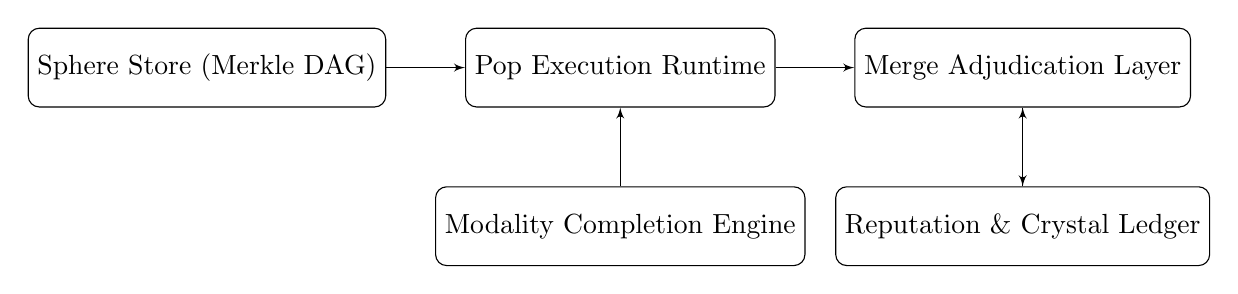
\begin{tikzpicture}[node distance=10mm, auto, >=latex']
  \tikzstyle{box} = [draw, rectangle, rounded corners, minimum width=28mm, minimum height=10mm]
  \node[box] (spheres) {Sphere Store (Merkle DAG)};
  \node[box, right=of spheres] (runtime) {Pop Execution Runtime};
  \node[box, right=of runtime] (merge) {Merge Adjudication Layer};
  \node[box, below=of runtime] (trans) {Modality Completion Engine};
  \node[box, below=of merge] (reputation) {Reputation \& Crystal Ledger};
  \draw[->] (spheres) -- (runtime);
  \draw[->] (runtime) -- (merge);
  \draw[->] (merge) -- (reputation);
  \draw[->] (trans) -- (runtime);
  \draw[->] (reputation) -- (merge);
\end{tikzpicture}
\end{document}
